% Chapter 3

\chapter{Analyzer Overview} % Main chapter title

\label{Chapter3}

\section{Theoretical Construction}
The development of our tool followed a structured, multi-step approach. As outlined in \capref{Chapter1}, to assess comment quality, it was necessary to categorize comments based on specific criteria.

\begin{figure}[ht]
	\centering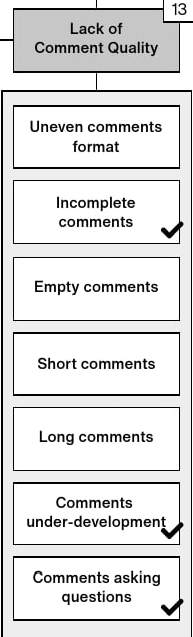
\includegraphics[height=350pt]{figs/goal-schema.PNG}
	\captionsetup{justification=centering}
	\caption{Categories of comments our study focuses on.}
	\label{fig:goal-schema}
\end{figure}

\begin{itemize}
	\item \textbf{Empty comments}: these provide no value or clarity and should be flagged for immediate attention.
	\item \textbf{Comments asking questions}: whether direct or implied, questions undermine the purpose of comments, which should provide clear and definitive information.
	\item \textbf{Short comments}: these fail to offer sufficient context or detail, leaving readers without a clear understanding of the code’s functionality or purpose.
	\item \textbf{Long comments}: excessively detailed comments can overwhelm readers, leading to confusion and obscuring the main point of the explanation.
	\item \textbf{Comments under development}: these temporary, technical comments are relevant only to active developers and must be regularly updated or removed as the system evolves.
	\item \textbf{Incomplete comments}: these lack full explanations, leaving gaps in the intended message, making them unclear or difficult to understand.
	\item \textbf{Uneven comments format}: inconsistent formatting or structure hinders readability, making it harder to follow and maintain the code. Comments should be clear, consistent, and well-structured to enhance usability.
\end{itemize}

\noindent We began with simpler detections, such as identifying empty comments and comments that posed questions. Established rules were applied to determine if a comment was empty or contained either direct or implied questions.

\noindent Next, we tackled short and long comments. To achieve this, we utilized NLTK \cite{NLTK}, a comprehensive suite for natural language processing. By tokenizing each comment, we measured its length to classify it as either too short or overly long.

\noindent For comments under development, we employed pattern recognition techniques. We incorporated technical keywords and common phrases used during development to detect these comments.

\noindent The detection of incomplete comments and uneven comments format was refined iteratively in a trial-and-error way, manually verifying results at each step. For incomplete comments, we initially performed a syntactic analysis to ensure the comments adhered to basic rules of English sentence structure. Subsequently, we built a classification system to categorize comments as single-line, multi-line, or documentation. For documentation comments, we verified consistency between the number of parameters in the comment and the corresponding source code, along with matching return types. Additionally, we introduced checks for single-line and multi-line comments to identify nonsensical or "gibberish" content, hence marking those that lacked clarity or coherence as incomplete.

\noindent Finally, for detecting uneven formatting, we flagged comments with irregular indentation, spacing, or annotation tag misuse, tailored to the programming language in use. This ensured that comments maintained proper structure, readability, and compliance with language-specific conventions.

\section{Logic Construction}\label{sec:logic-construction}

\begin{figure}[ht]
	\centering\includegraphics[width=400pt]{figs/whole-architecture.PNG}
	\captionsetup{justification=centering}
	\caption{General view on the tool's architecture.}
	\label{fig:whole-architecture}
\end{figure}

\noindent Our tool's architecture is structured in multiple layers. For clarity, we begin by outlining the foundational components.

\begin{figure}[ht]
	\centering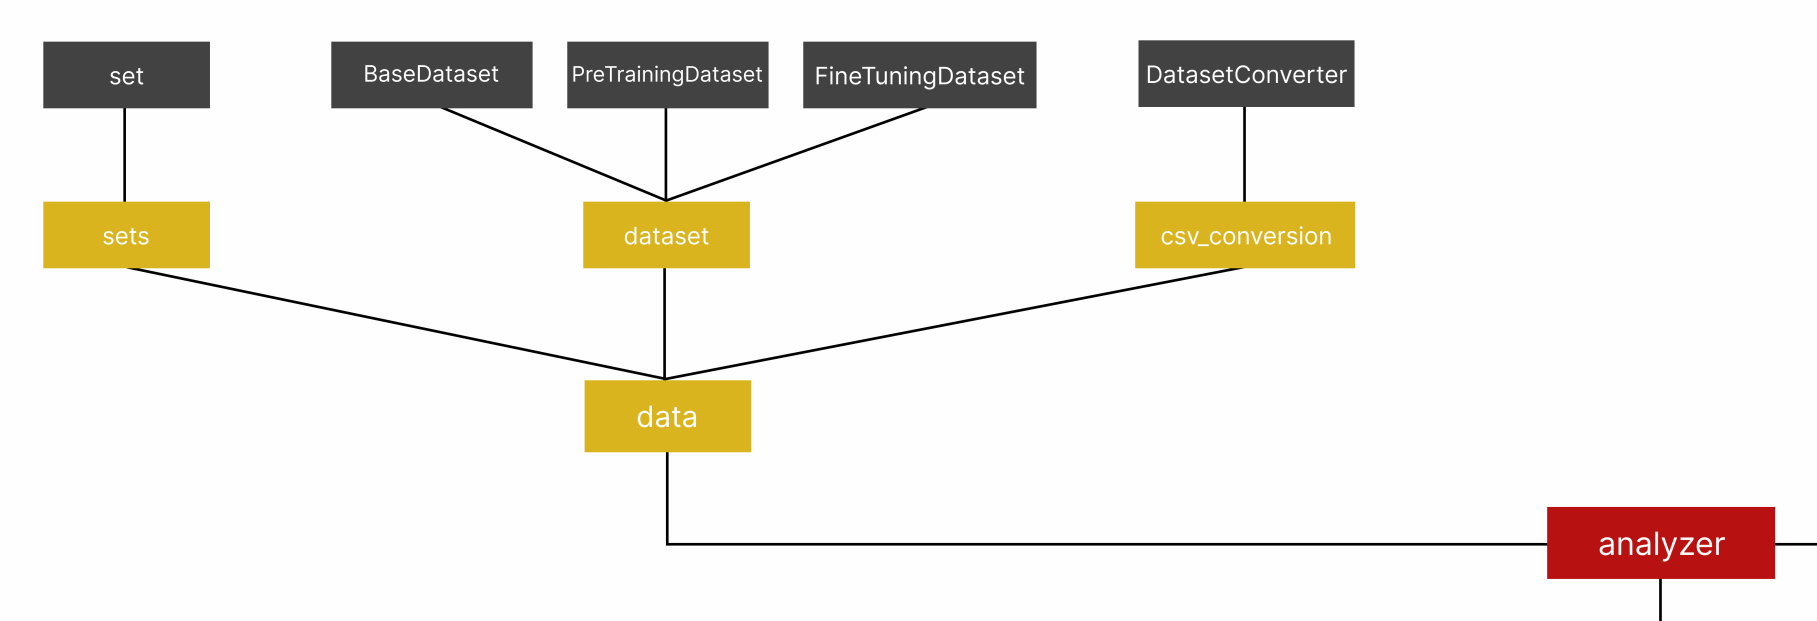
\includegraphics[width=400pt]{figs/zoom-data.PNG}
	\captionsetup{justification=centering}
	\caption{Zoom on the tool's data package.}
	\label{fig:zoom-data}
\end{figure}

\noindent The "data" package defines the supported dataset file formats our tool is able to read, provides a common interface for loading and working with datasets, and handles dataset format conversion when necessary.

\newpage
	
\begin{figure}[ht]
	\centering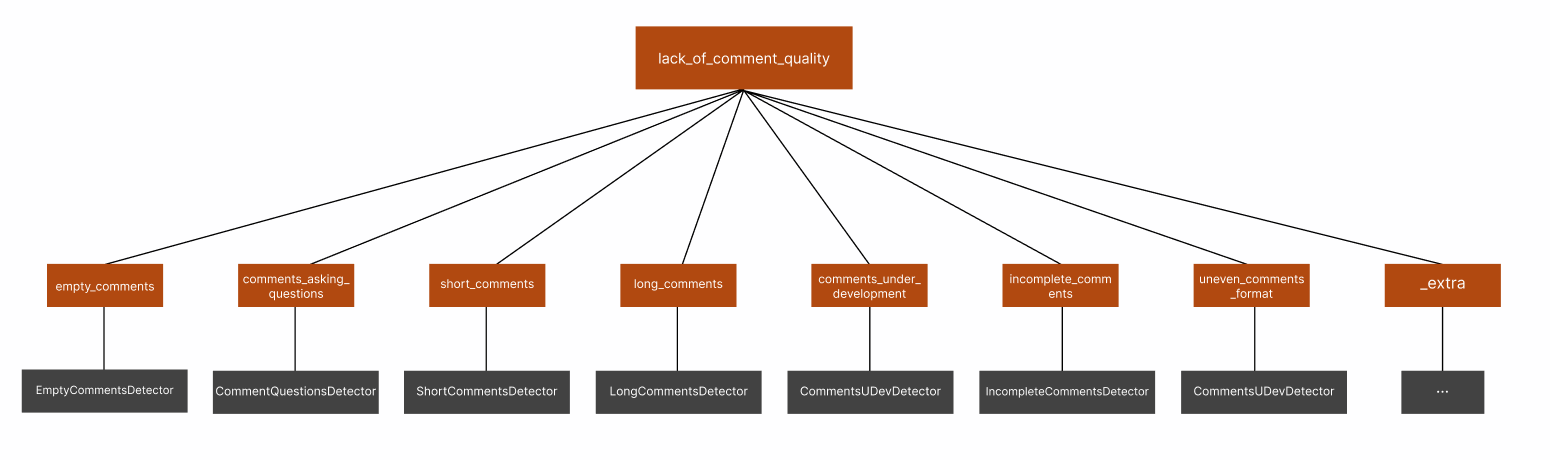
\includegraphics[width=465pt]{figs/zoom-cmsquality.PNG}
	\captionsetup{justification=centering}
	\caption{Zoom on lack of comments quality package.}
	\label{fig:zoom-cmsquality}
\end{figure}
	
\noindent The "smells" package houses several detectors, but for the purpose of this work, we will focus solely on those that align with the scope of our study. We begin by detailing essential components without which our tool would not function.

\begin{figure}[ht]
	\centering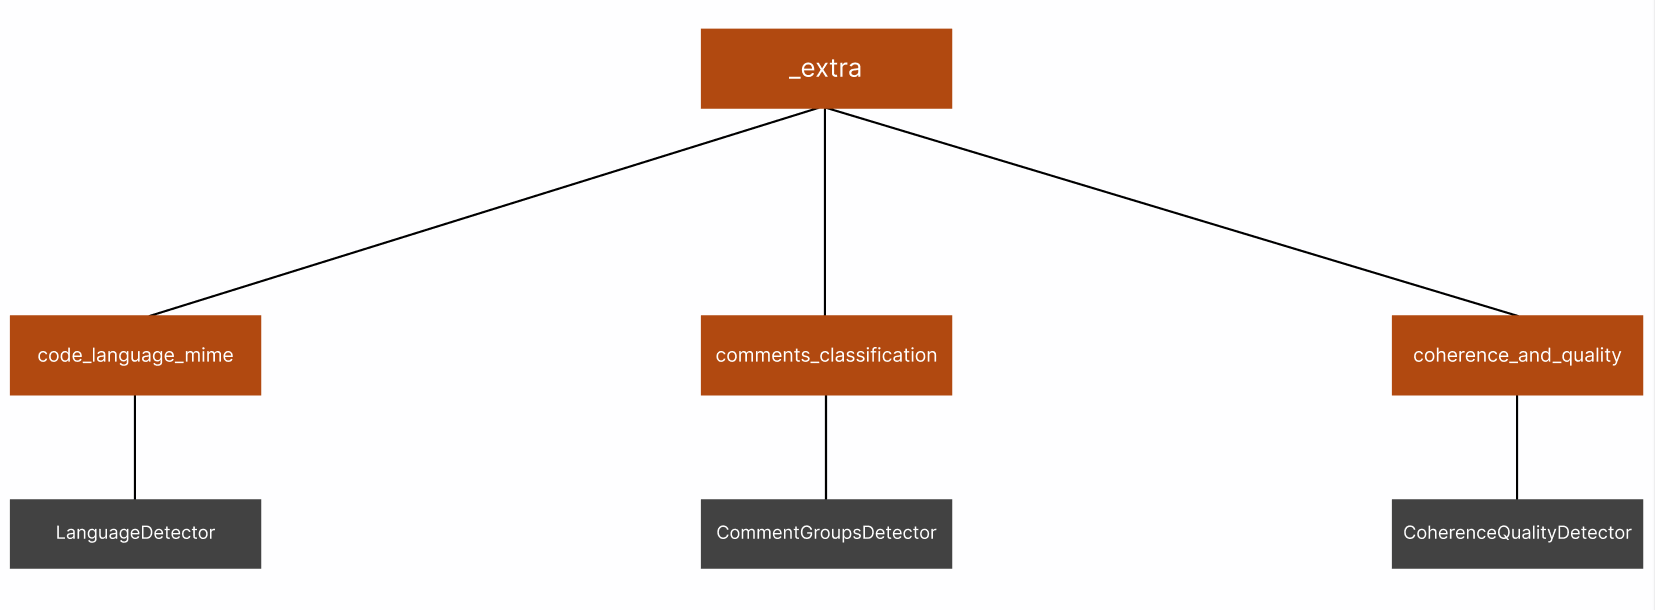
\includegraphics[width=400pt]{figs/zoom-extra.PNG}
	\captionsetup{justification=centering}
	\caption{Zoom on extra sub-package.}
	\label{fig:zoom-extra}
\end{figure}

\noindent Initially, we aimed for the tool to be language-agnostic, meaning it would work with all programming languages. While this is true for some detectors, it’s not feasible for all. As a result, we introduced a programming language detector, represented by the "code\_language\_mime" sub-package and its corresponding \textit{LanguageDetector} class.

\noindent The \textit{CommentGroupsDetector} scans all comments in the input database and categorizes them as single-line, multi-line, or documentation comments. This classification is crucial for enabling the incomplete comments detector and the uneven comments format detector to function correctly.

\noindent An additional detector, the \textit{CoherenceQualityDetector}, resides in the 

\noindent "coherence\_and\_quality" sub-package. This detector was developed while researching comment completeness, but it doesn’t strictly relate to incomplete comments, so it was placed in a separate package. The detector evaluates comments based on the following criteria:
	\begin{itemize}
		\item \textbf{Language (L)}: ensures the comment is not written in a mix of different languages.
		\item \textbf{Clarity (C)}: uses NLP techniques to assess the readability of the comment.
		\item \textbf{Relevance (R)}: verifies that the comment accurately describes the specific code constructs it’s meant to explain.
		\item \textbf{Brevity (B)}: checks if the comment avoids unnecessary repetition or wordiness.
		\item \textbf{Context (X)}: determines whether the comment provides sufficient explanation for understanding the code.
	\end{itemize}
If a comment meets all these criteria, it is considered coherent. Otherwise, it is flagged as incoherent.
	
\section{Heuristics Used}
We will list the heuristics for each category related to the lack of comment quality.
In all cases, the following notations can be used: let \textit{C} be a code block to be analyzed, let \textit{M} be the MIME type of the code block, let \textit{extract(C, M)} be a method that extracts comments from \textit{C} based on MIME type \textit{M}.

\noindent Let \textit{comment(i)} represent the i-th comment in the extracted list of comments from \textit{C}.

\noindent Let \textit{text(i)} represent the text of the i-th comment.

\subsection{Empty Comments}
\noindent Let isEmpty\textit{(i)} be the empty comment condition: 
\begin{equation*}
	\textbf{isEmpty}(i) = \begin{cases}
		1, & \text{if } \text{ strip(text\textit{(i)}) = ""} \\
		0, & \text{ otherwise}
	\end{cases}
\end{equation*}
where \textit{strip(text(i))} removes all leading and trailing whitespace from the comment.

\noindent We define the function \textit{F(C, M)} that evaluates if the code block \textit{C} contains empty comments based on the MIME type \textit{M}:
\begin{equation*}
	F(C, M) = \begin{cases}
		1, & \text{if } \exists i \text{ such that } \text{isEmpty}(i) = 1 \text{ for any comment } i \in \text{extract}(C, M) \\
		0, & \text{ otherwise}
	\end{cases}
\end{equation*}

\subsection{Comments Asking Questions}
Define the set of interrogative phrases as:
\begin{equation*}
	I = \text{\{"why", "how", "what is", "what\\'s", "where\\'s", "where is", "where are", "how long"\}}
\end{equation*}

\noindent Then, the condition is isQuestion\textit{(i)}, where:
\begin{equation*}
	\textbf{isQuestion}(i) = \begin{cases}
		1, & \text{if } \text{text}(i) \text{.endswith("?")} \vee \text{text}(i) \text{.startswith}(I) \\
		0, & \text{ otherwise}
	\end{cases}
\end{equation*}

\noindent We define the function \textit{F(C, M)} that evaluates if the code block \textit{C} contains any questions based on the MIME type \textit{M}:
\begin{equation*}
	F(C, M) = \begin{cases}
		1, & \text{if } \exists i \text{ such that } \text{isQuestion}(i) = 1 \text{ for any comment } i \in \text{extract}(C, M) \\
		0, & \text{ otherwise}
	\end{cases}
\end{equation*}

\subsection{Short Comments}
Let T\textit{(i)} = tokenize(text\textit{(i)}) be the list of tokens in the i-th comment.

\noindent Let us define a threshold for short comments as k = 5 (maximum number of tokens).

\noindent Let us define the short comments condition as isShort\textit{(i)}, where:
\begin{equation*}
	\textbf{isShort}(i) = \begin{cases}
		1, & \text{if } \mathrm{|T|}_{i} \le k \\
		0, & \text{ otherwise}
	\end{cases}
	
	\noindent \text{where} \mathrm{|T|}_{i} \text{ represents the number of tokens in the i-th comment.}
\end{equation*}

\noindent We define the function \textit{F(C, M)} that evaluates if the code block \textit{C} contains any short comments based on the MIME type \textit{M}:
\begin{equation*}
	F(C, M) = \begin{cases}
		1, & \text{if } \exists i \text{ such that } \text{isShort}(i) = 1 \text{ for any comment } i \in \text{extract}(C, M) \\
		0, & \text{ otherwise}
	\end{cases}
\end{equation*}

\subsection{Long Comments}
The heuristic is similar to that used for short comments, but in the first case, the comparison is reversed.
It is inspired by the work of \textit{Steidl et al.} \cite{steidl2013}, but our approach uses tokens rather than words.

\noindent Let us define a threshold for long comments as k = 30 (minimum number of tokens).

\noindent Let us define the long comments condition as isLong\textit{(i)}, where:
\begin{equation*}
	\textbf{isLong}(i) = \begin{cases}
		1, & \text{if } \mathrm{|T|}_{i} \ge k \\
		0, & \text{ otherwise}
	\end{cases}
	
	\noindent \text{where} \mathrm{|T|}_{i} \text{ represents the number of tokens in the i-th comment.}
\end{equation*}

\begin{equation*}
	F(C, M) = \begin{cases}
		1, & \text{if } \exists i \text{ such that } \text{isLong}(i) = 1 \text{ for any comment } i \in \text{extract}(C, M) \\
		0, & \text{ otherwise}
	\end{cases}
\end{equation*}

\subsection{Comments Under Development}
This heuristic is inspired by the work of \textit{Shi et al.} \cite{buildingRock}.

\noindent Let us define the following sets of keywords:
	\begin{itemize}
		\item \textit{P} = placeholder keywords, e.g., "Description of the Method", "Logic goes here".
		\item \textit{N} = temporary notes, e.g., "Add more info here", "Temporary fix for issue".
		\item \textit{D} = vague descriptions, e.g., "To be documented", "Work in progress".
		\item \textit{R} = redundant keys, e.g., "Opens a file", "Calls the method".
		\item Let $\mathrm{R}_{M}$ represent a set of MIME-type specific patterns to detect commented methods (e.g., method definitions in Java, Python, etc.).
	\end{itemize}
	
\noindent Let\begin{math*}
	regexMatch(\textit{i, P, N, D, R, } \mathrm{R}_{M})
\end{math*} be a function that checks whether any of the patterns defined by \begin{math*}\textit{P, N, D, R, } \mathrm{R}_{M} \end{math*} match the comment text \textit{text(i)}.

\noindent Let us define the under development condition as isUnderDev\textit{(i)}, where:
\begin{equation*}
	\textbf{isUnderDev}(i) = \begin{cases}
		1, & \text{if } \text{regexMatch(i, P, N, D, R, }  \mathrm{R}_{M}) = 1 \\
		0, & \text{ otherwise}
	\end{cases}
\end{equation*}

\noindent We define the function \textit{F(C, M)} that evaluates if the code block \textit{C} contains any comments indicative of being "under development" based on the MIME type \textit{M}:
\begin{equation*}
	F(C, M) = \begin{cases}
		1, & \text{if } \exists i \text{ such that } \text{isUnderDev}(i) = 1 \text{ for any comment } i \in \text{extract}(C, M) \\
		0, & \text{ otherwise}
	\end{cases}
\end{equation*}

\subsection{Incomplete Comments}
Let \textit{SML} represent groups of comments classified by \textit{CommentGroupsDetector} into single-line or multi-line.

\noindent Let \textit{DOC} represent the group of comments classified as documentation by \textit{CommentGroupsDetector}.

\noindent Let us assume we are able to detect different types of comment formats (e.g., \textit{Google}, \textit{NumPy}, \textit{ReST}, \textit{epytext}, \textit{Javadoc}) based on the detected structure of comments and the programming language.

\noindent For single-line and multi-line comments, first we have to check whether a comment is written in English.
\begin{equation*}
	\mathrm{F}_{english}(comment) = \begin{cases}
		1, & \text{if the comment} \in \textit{SML } \wedge \text{ is classified as English} \\
		0, & \text{if the comment} \in \textit{SML } \text{ but is in a different language}
	\end{cases}
\end{equation*}

\noindent Then, we check the syntactic completeness of a comment by verifying if each sentence contains a subject and a predicate, assuming the comment $\in$ \textit{SML}.
\begin{equation*}
	\mathrm{F}_{syntax}(comment) = \begin{cases}
		1, & \text{if  } \exists \text{sentence} \in \text{comment syntactically incomplete} \\
		0, & \text{if all sentences are complete}
	\end{cases}
\end{equation*}

\noindent Lastly, we evaluate whether a comment, assumed $\in$ \textit{SML}, is gibberish using a pre-trained model \cite{gibberishDetector} that classifies comments into various categories.
\begin{equation*}
	\mathrm{F}_{gibberish}(comment) = \begin{cases}
		1, & \text{if  } \exists \text{sentence} \in \text{comment classified as gibberish} \\
		0, & \text{if all sentences are clean}
	\end{cases}
\end{equation*}

\noindent For documentation comments, we must check if a comment is missing any critical part in annotation tags (wrong number of params, lack of return type) compared to the code block it refers to.

\noindent Let $\mathrm{P}_{comment}$ represent the number of @param annotations in the comment, assuming comment $\in$ \textit{DOC}.

\noindent Let $\mathrm{R}_{comment}$ represent the number of @return annotations in the comment (which can be only 0 or 1), assuming comment $\in$ \textit{DOC}.

\noindent We check the number of parameters in the function signature.
\begin{equation*}
	\mathrm{F}_{params}(C) = \begin{cases}
		n, & \text{if the function has parameters} \\
		0, & \text{if no parameters exist}
	\end{cases}
\end{equation*}

\noindent Then, we check the return type in the function signature.
\begin{equation*}
	\mathrm{F}_{return}(C) = \begin{cases}
		1, & \text{if it returns a value other than void
		} \\
		0, & \text{if it returns void or no return type is found}
	\end{cases}
\end{equation*}

\noindent To conclude we can say that, for a single-line or multi-line comment to be incomplete, the following conditions must be met:
	\begin{enumerate}
		\item The comment is in English.
		\item The comment is syntactically incomplete.
		\item The comment contains gibberish.
	\end{enumerate}
	
\noindent Thus, the overall incompleteness function for single-line or multi-line comments $\mathrm{F}_{incomplete}^{\textit{ SML}}$ can be expressed as:
\begin{equation*}
	\mathrm{F}_{incomplete}^{\textit{ SML}} = \begin{cases}
		1, & \text{if } \mathrm{F}_{english}(comment) = 1 \wedge \mathrm{F}_{syntax}(comment) = 1 \wedge \mathrm{F}_{gibberish}(comment) = 1 \\
		0, & \text{otherwise}
	\end{cases}
\end{equation*}

\noindent For a documentation comment to be incomplete, it means there is either a mismatch between the number of \textit{@param} annotations and the actual number of parameters, or a mismatch between the presence of a \textit{@return} annotation and whether the function actually returns a value.

\noindent This implies that the incompleteness function for documentation comments $\mathrm{F}_{incomplete}^{\textit{ DOC}}$ can be expressed as:
\begin{equation*}
	\mathrm{F}_{incomplete}^{\textit{ DOC}} = \begin{cases}
		1, & \text{if } \mathrm{P}_{comment} \ne \mathrm{F}_{params}(C) \\
		1, & \text{if } \mathrm{R}_{comment} = 1 \wedge \mathrm{F}_{return}(C) = 0 \\
		1, & \text{if } \mathrm{R}_{comment} = 0 \wedge \mathrm{F}_{return}(C) = 1 \\
		0, & \text{otherwise}
	\end{cases}
\end{equation*}

\subsection{Uneven Comments Format}
Let \textit{SL} be the group of single-line comments, \textit{ML} the group of multi-line comments and \textit{DOC} the group of documentation comments.

\noindent Let \textit{SF} be the single-line way of comment formatting (e.g, // in \textit{Java}, # in \textit{Python}).

\noindent Let \textit{MF} be the multi-line way of comment formatting (e.g, /* or /** in \textit{Java}, ''' or """ in \textit{Python})

\noindent Let \textit{TAGS} be an array of commonly used HTML tags in Javadoc comments.

\noindent Let \textit{S} be a sentence $\in$ comment.

\noindent Let spaces\textit{(S)} represent the number of spaces in that sentence.

\noindent Let \textit{K} be the maximum number of spaces allowed per sentence.

\noindent We have a function that checks whether there are too many spaces (more than \textit{K} consecutive) in any sentence from the comment, which could indicate indentation issues.
\begin{equation*}
	\mathrm{F}_{spacing}(comment) = \begin{cases}
		1, & \text{if } \exists S \in comment : spaces(S) > K \\
		0, & \text{otherwise}
	\end{cases}
\end{equation*}

\noindent Single-line and multi-line comments should not contain any HTML tags, as they are treated as plain text.
Assuming comment $\in$ \textit{SL} $\vee$ comment $\in$ \textit{ML}:
\begin{equation*}
	hasTags(comment) = \begin{cases}
		1, & \text{if } \exists T \subset TAGS : T \in comment \\
		0, & \text{otherwise}
	\end{cases}
\end{equation*}

\noindent For a single-line comment to be uneven, we check the number of spaces or if it matches the multi-line format.
\begin{equation*}
	\mathrm{F}_{uneven}^{\textit{ SL}}(comment, MF) = \begin{cases}
		1, & \text{if } \mathrm{F}_{spacing} = 1 \vee hasTags(comment) = 1 \vee match(comment, MF) \\
		0, & \text{otherwise}
	\end{cases}
\end{equation*}

\noindent For a multi-line comment to be uneven, we do the opposite.
\begin{equation*}
	\mathrm{F}_{uneven}^{\textit{ ML}}(comment, SF) = \begin{cases}
		1, & \text{if } \mathrm{F}_{spacing} = 1 \vee hasTags(comment) = 1 \vee match(comment, SF) \\
		0, & \text{otherwise}
	\end{cases}
\end{equation*}

\noindent For documentation comments, we have a function that checks for irregularities in the use of annotation tags (e.g, wrong indentation, empty annotation, wrong token after annotation, ends with annotation). In particular, if the annotation is \textit{@author} and the following token is a verb, it makes no sense. If the annotation is followed by a redundant token (e.g, @return nothing), it should be avoided.

\noindent Let \textit{RDT} be an array of possible redundant words after an annotation (e.g, author, param, nothing, none, void).
Assume comment $\in$ \textit{DOC}, and the current token is an annotation.
\begin{equation*}
	\mathrm{F}_{irr}^{\textit{ DOC}}(comment) = \begin{cases}
		1, & \text{if } \text{token} = \textit{'@author'} \wedge \text{token\textit{.next}} \in \text{'VERB'} \\
		1, & \text{if } isSpace(token.next) = 1 \wedge \mathrm{F}_{spacing} = 1 \\
		1, & \text{if } isEmpty(token.next) = 1 \\
		1, & \text{if } token.next \in RDT \\
		0, & \text{otherwise}
	\end{cases}
\end{equation*}
